\documentclass[12pt, fleqn]{article}
\usepackage[utf8]{inputenc}
\usepackage[top=0.85in, bottom=0.85in, left=0.85in, right=0.85in]{geometry}
\usepackage{graphicx}
\usepackage{amsmath}
\usepackage{amssymb}
\usepackage{setspace}
%\singlespacing
\onehalfspacing
%\doublespacing
%\setstretch{1.1}


\title{DroiDTN: Optimizing Bandwidth over Wifi and 3G on Smartphones}
\author{Shreshth Singhal}
\date{May 6, 2013}

\begin{document}

\maketitle

\begin{abstract}
  Lorem ipsum dolor sit amet, consectetur adipisicing elit, sed do eiusmod 
  tempor incididunt ut labore et dolore magna aliqua. Ut enim ad minim veniam, 
quis nostrud exercitation ullamco laboris nisi ut aliquip ex ea commodo consequat. 
Duis aute irure dolor in reprehenderit in voluptate velit esse cillum dolore eu fugiat 
nulla pariatur. Excepteur sint occaecat cupidatat non proident, sunt in culpa qui officia 
deserunt mollit anim id est laborum.
\end{abstract}

%%%%%%%%%%%%%%%%%%%%%%%%%%%%%%%%%%%%%%%%%
%%%%%%%%%%%%%%%% SECTION %%%%%%%%%%%%%%%%%%
%%%%%%%%%%%%%%%%%%%%%%%%%%%%%%%%%%%%%%%%%

\section{Introduction}

Worldwide, the use of smartphones is becoming ubiquitous. One of the primary 
advantages of using smartphones over their ``non-smart" counterparts 
is the ability to access the internet, either through wireless (wifi) or 
cellular data networks (3G, 4G LTE etc.). More and more smartphones are available that are leveraging 
these networks to bring more and more content to users - be it through apps, 
services, or directly browsing the internet.

%%%%%%%%%%%%%%%%%%%%%%%%%%%%%%%%%%%%%%%%%
%%%%%%%%%%%%%%%% SUBSECT %%%%%%%%%%%%%%%%%%
%%%%%%%%%%%%%%%%%%%%%%%%%%%%%%%%%%%%%%%%%

\subsection{Motivation: comparison of wifi and 3G}

As smartphones have proliferated,  so have cellular data networks. We know these through 
various names - 3G, 4G LTE etc. (we will refer to these collectively as 3G for short from now on).
 However, data networks have imposed infrastructural limits because of 
which users do not have access to unlimited network usage. We see this in the 
way that data plans offered by network providers are moving away from the 
concept of ``unlimited" plans towards expensive plans, data caps and throttling.\cite{att-data-plans}\cite{verizon-data-plans}
Further, data networks are not available 
uniformly everywhere. There are plenty of pockets where data connectivity is 
poor or nonexistent.\cite{att-coverage}\cite{verizon-coverage} Data networks also have an associated cost as reflected in 
data plans. This is usually a package cost up to a certain limit of data usage, 
and a per-byte fee thereafter. Data networks have also been shown to be less 
power-efficient than wifi, due to lower transfer rates (although the power usage
rate over time is around the same)\cite[p. 8]{lee-2012}

On the other hand, wifi tends to be free, or at the very least, cheaper than 
data networks. wifi networks also usually don't have aggressive caps or thresholds 
on their usage, and don't face data throttling problems. However, it is important to 
note that wifi is not ubiquitous either. Wifi routers are stationary and limited 
in their range, considerably more so than data networks which are provided 
through long-range cellular towers. Further, installing wifi infrastructure is still
quite expensive.\cite[p. 105]{raman-2007} Many people face the problem of not being 
able to connect to wifi on the move. An even more annoying problem is when our 
phones connect to a wifi network but are unable to send or receive data at a 
usable rate because of poor connection.

Therefore, we can see that neither wifi nor 3G can function perfectly on their 
own. They have differing costs, availability and bandwidth, which themselves 
differ across different locations and times. The ideal goal would be to provide 
the user with good, usable network connections as often as possible, in a 
manner that reduces the cost to them and provides them with a good experience.
Therefore, smartphones should be capable of switching 
between wifi and data networks smartly in a manner that minimizes cost, while at 
the same time ensuring the quality of service is good.

%\bigskip
%\textbf{Todo:}
%\begin{itemize}
% \item {write about current ways of using wifi and 3G together}
% \item {add more detail about wifi vs 3g comparisons and cite papers for results}
%\end{itemize}

%%%%%%%%%%%%%%%%%%%%%%%%%%%%%%%%%%%%%%%%%
%%%%%%%%%%%%%%%% SUBSECT %%%%%%%%%%%%%%%%%%
%%%%%%%%%%%%%%%%%%%%%%%%%%%%%%%%%%%%%%%%%

\subsection{Problem - Network Scheduling}

We have seen that wifi and 3G do not work best alone. Our goal therefore is to 
leverage them in combination in a way that makes the user happy. The characterizations 
of wifi and 3G above are an indication of the direction we should take to be able to 
provide a better experience for the user - we need to focus on \textbf{quality of service} 
and \textbf{limiting cost}. 

As we have seen before, 3G tends to be more expensive than wifi. 
Offloading network traffic to wifi whenever possible is hence an ideal goal. It 
may seem trivial to do so - just use wifi when it is available and 3G otherwise.
However, there are improvements we can make to this trivial solution. 
We can leverage the fact that certain network traffic on 
smartphones is \textbf{delay-tolerant}. This means that we can delay 3G traffic in the 
hopes of waiting for wifi to show up, as long as it doesn't affect the user's 
experience. An example of this is 
the case of e-mail syncing. E-mail clients on phones constantly synchronize webmail in the 
background. Oftentimes, however, this process can be delayed, since the user does not 
check email all the time, and would not notice the difference if email came in a minute later.

There are complications that arise because we want to provide the user good 
quality of service. Because of this, we obviously cannot delay traffic 
immediately affects the user - for example, if the user is watching a video or clicks on a link on
a website, we cannot delay it since the user is directly interacting with the 
phone and cares about getting results immediately. Further, we also do not want 
to offload to wifi in cases where the wifi signal is poor and would result in a 
bad experience for the user.

Note that we are focusing here on traffic that is produced by the phone, i.e. 
network traffic leaving the phone. This is because, in most common applications, 
even if the phone needs to receive some information, it is not done unilaterally 
by the server. Rather, the phone makes a request to the server for information, 
and the server responds to this request. For example, email syncing is done by 
the phone pinging the webmail server to find out if any new email has been 
received. This simplifies the model since we only need to focus on the network
traffic generated by the phone, and can abstract away the traffic received by 
the phone as responses to the phone's requests, and hence part of the same 
network transaction.

Therefore, our \textbf{problem statement} resolves to the following: we need to 
schedule network traffic generated by the phone through either wifi or 3G in a 
manner that minimizes cost, while at the same time ensuring good quality of 
service. In effect, this is a \textbf{network scheduling problem}. 
To this end, we can do many smart things, such as leveraging delay 
tolerance of some network traffic to avoid using 3G and hence reducing cost 
without affecting the user.
 
%%%%%%%%%%%%%%%%%%%%%%%%%%%%%%%%%%%%%%%%%
%%%%%%%%%%%%%%%% SECTION %%%%%%%%%%%%%%%%%%
%%%%%%%%%%%%%%%%%%%%%%%%%%%%%%%%%%%%%%%%%

\section{Related work}
\label{related-work}

A paper by Ozlem Bilgir Yetim and Margaret Martonosi in CHANTS '12 talks about a 
theoretical framework for optimizing network traffic on smartphones between wifi 
and 3G. The framework requires perfect knowledge about all network data streams on the
smartphone, and about the availability of wifi and 3G in the future. Given this 
knowledge, they resolve the problem to a mixed-integer linear programming 
problem, where they try to minimize the cost of traffic sent over 3G, subject to 
the constraints defined by the data streams and network availability. The linear program 
assigns the optimal network to be used by each data unit in order to minimize 
this cost.\cite{ozlem-2012} This method makes intuitive sense - they have  
perfect knowledge about how much data the apps are going to generate in the future, and 
also about the wifi and 3G characteristics at all those times in the future. 
They also assume knowledge of delay tolerance of the network data. Given all 
this knowledge, they can schedule all network data over wifi and 3G in a manner 
that reduces cost

Another paper by Lee et al. talks about the real-world performance of wifi 
offloading. They conclude that wifi offloading without taking into account delay 
tolerance is quite effective in itself, but can be made more efficacious by 
adding delay (they add a constant delay to network traffic). They further 
propose a framework similar to the above to generate network traffic and measure 
the effect of offloading under delay.\cite{lee-2012}

\bigskip
\textbf{Todo:}
\begin{itemize}
  \item Expand this with new papers
  \item Also include overview of Serval and more in-depth look at Ozlem's since 
  these relate to my work greatly
\end{itemize}

%%%%%%%%%%%%%%%%%%%%%%%%%%%%%%%%%%%%%%%%%
%%%%%%%%%%%%%%%% SECTION %%%%%%%%%%%%%%%%%%
%%%%%%%%%%%%%%%%%%%%%%%%%%%%%%%%%%%%%%%%%

\section{Overview of solution}
\label{overview}

\subsection{Leveraging delay tolerance - theoretically}

The most nebulous part of the solution as described above is the notion of 
\textbf{delay tolerance}. Network traffic is delay tolerant if it can withstand some 
delay to its transmission without affecting the user. Note that not all 
delay-tolerant traffic is equal - some applications' traffic can be delayed more than others. 
For example, email syncing can be delayed for times on the order of minutes, since users 
tend to check for new email infrequently. [CITE?] On the other hand, 
video streaming applications have a much shorter threshold - we can only delay 
traffic as long as the video frame-buffer is not close to being empty, since 
the user would be affected if the buffer became empty and the video stopped 
playing. Delay tolerance is therefore defined per-application and is a 
measure, in seconds, of how much that application's traffic can be delayed. 

This gives rise to a few questions. How exactly do we tell what network traffic is tolerant to 
delay? How much should we delay such traffic in the hopes of getting wifi soon?
How do we quantify the ``hope" of getting wifi soon? The intuition behind my method 
requires perfect knowledge about two things:
\begin{enumerate}
  \item \emph{network traffic}: How much network traffic is going to be 
  generated by the phone for all times in the future? What is the nature of this 
  network traffic - how much of it is tolerant to delay, and how much must be 
  sent immediately? What is the individual delay tolerance of each of the 
  applications that are producing network traffic?
  \item \emph{availability of wifi and 3G}: What is the nature of wifi and 3G 
  that the user (and the phone) is going to experience at all times/all 
  locations? What is the speed, signal strength and availability of these 
  networks?
\end{enumerate}
It is easy to see that with perfect knowledge of these things, we can schedule 
wifi and 3G in an optimal manner. We know exactly the sort of traffic we are
going to see, and we know the exact nature of the networks that we are going to 
be sending them over. We can therefore schedule traffic that is not delay 
tolerant over whatever network is available at the time the traffic needs to be 
sent. For traffic that can be delayed, we can gauge whether it is possible to 
wait and send it over wifi, and still remain within the limits of its delay 
tolerance. If we cannot do so, we can just send it over 3G. 

\subsection{A real solution - machine learning}

In a real system, we are not going to be presented with this perfect 
information. Therefore, we must learn this from past measurements, in essence 
reducing this to a machine learning problem. Corresponding to the two aspects of 
perfect information required (from the previous section), we have two sources of 
past information we can learn from, so as to emulate this perfect information:
\begin{enumerate}
     \item \emph{application delay tolerance estimation}: We can
     track the past network usage of each application on the smartphone. From 
     this, we can learn the delay tolerance of the app, for example, by looking
     at the time the app usually takes between sending successive requests. This 
     will give us an approximate handle on how long the app's traffic can be 
     delayed.
     
     Then, when we are actually scheduling traffic, we can look at which app 
     generated the traffic, and use its delay tolerance estimate to figure out 
     if we can delay it or not.
     
    \item \emph{future wifi prediction}: We can track the wifi and 3G 
    availability and quality at different physical locations as the user of the phone moves 
    around. Then, when we are scheduling 
    traffic, we can look at the user's current location and direction of motion 
    to predict how long it will take them to be in range of usable wifi. If the 
    traffic is delay tolerant enough to wait for this time, then we can delay 
    the traffic, otherwise we can send it immediately over 3G. Of course, if our 
    prediction of the time required to reach wifi was incorrect, we need to 
    failover and immediately send the traffic over 3G. 
    
    Note that this method will be more successful the more dense and accurate 
    our mapping of wifi and 3G in different locations is. Therefore, it would 
    make sense to share this data across all users so as to collaboratively have 
    a better understanding of the network map.
\end{enumerate}

\subsection{Putting it all together}

After gaining a high-level understanding of our problem and possible insights on 
tackling it in the previous sections, we can see that there are multiple pieces that 
must be built:

\begin{itemize}
  \item \textbf{Policy}: For every network packet that we see, how much should 
  we delay it? This is what we will refer to as the ``policy" for delaying 
  traffic. This policy is determined by the two different measurements that 
  we described in the previous section:
  \begin{enumerate}
     \item An \emph{application delay tolerance estimator}: This estimator 
     tracks the network usage statistics of each application on the smartphone, 
     to learn the delay tolerance of each app. 
     
    \item A \emph{time-to-wifi predictor}: This predictor tracks wifi and 3G 
    signal strength and availability at different places as the user walks around 
    with their phone. From these, it can learn to predict the time it will take 
    to get in range of wifi, given the user's current location and direction of 
    motion.
  \end{enumerate}
  
  Using these measurements, we can determine a policy to delay traffic. One that immediately
  springs to mind would be to delay traffic if 
  \[\textrm{delay tolerance} \geq \textrm{time-to-wifi} \]
  However, it is important to note that this is not the only sensible policy. 
  Other policies like a fixed delay or zero delay for all traffic may also make sense in certain 
  cases. For example, if our map of wifi and 3G in different locations is very sparse, 
  then it is likely that our time-to-wifi predictor will be inaccurate. Because 
  of this, it may make sense to replace the time-to-wifi value with infinity or double 
  each value just to be safe. Equivalently, if we don't have much confidence in 
  our application delay tolerance estimator, then we can just replace the delay 
  tolerance values with zero or some small fixed value just to be safe. 
  
  \item \textbf{Mechanism}: Now that we have a policy for when to delay network 
  traffic, and how long to delay it, we still need to set up the mechanism to make the delaying 
  work. This ``mechanism" refers to some actual piece of code that will run on 
  the smartphone and delay packets of data for some time, depending on the 
  policy. This mechanism could be run in many ways, in the application level, or 
  within the OS. We want to try and ensure that the mechanism runs in a way that 
  makes it easy to program and invisible to the user. We also want to ensure that we
  abstract away the complexities as much as we can from application developers 
  who are going to be writing apps which generate network traffic.
\end{itemize}

\noindent Therefore, the pieces of the solution as described are:

\newpage
\begin{figure}[htp]
\centering
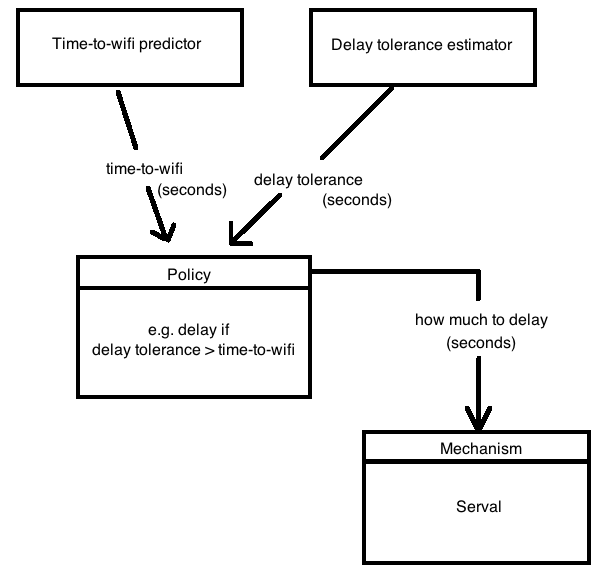
\includegraphics[scale=0.8]{img/method-flowchart.png}
\caption{Method\label{fig-method-flowchart}}
\end{figure}
\medskip

%%%%%%%%%%%%%%%%%%%%%%%%%%%%%%%%%%%%%%%%%
%%%%%%%%%%%%%%%% SECTION %%%%%%%%%%%%%%%%%%
%%%%%%%%%%%%%%%%%%%%%%%%%%%%%%%%%%%%%%%%%
\newpage
\textbf{BELOW IS WORK IN PROGRESS}
\newpage

\subsection{Setting}

I will be working with an Android smartphone - specifically a Galaxy Nexus 
running Android 4.1.1 (Jelly Bean API 16). The setting for my experiments is the 
Princeton University campus. The campus is characterized by wifi that is open 
and available freely in all buildings and also in a lot of open spaces. However, 
there are certain stretches which do not have wifi or suffer from poor 
connectivity. 3G is available across campus on the AT&T network which 
I will be using for testing. 

This small geographic area therefore has a wide array of wifi profiles, and the 
prevalence of 3G allows it to be catchall or a fallback for network traffic in 
places where wifi is not available. This makes it a good location for testing 
our system - we can easily test if the app aggressively delays traffic in 
the places where wifi is not available, since it is quite likely that the user 
will be in range of wifi soon (because wifi is quite widely available).

I will be testing with an open source email client for Android, called K-9. This 
is the app that I will be testing with for determining delay tolerance, 
and testing the policy. It will also be used for data collection

%\bigskip
%\textbf{Todo: campus map picture, possibly with areas that don't have wifi outlined.}

\subsection{Approach}
\label{overview-approach}

There are multiple approaches which can be taken to implement the policy and 
mechanism as described above. 
\begin{itemize}
    \item \emph{Application-level}: One way would be to build a system 
    entirely on the application-level, without going into the kernel/OS. Firstly,
    we would be to build the \emph{time-to-wifi predictor} as an app for 
    the smartphone, which would store all the information about wifi and 3G 
    at different locations, and learn from this data to predict time-to-wifi.
    
  Each other app, before making a network request, would ask this app for how 
  much time it will take to be in range of wifi. Then the apps can internally 
  make judgements, based on their own known delay tolerance, about whether to 
  delay their traffic or not. We therefore place the \emph{delay tolerance estimator} in the apps 
  themselves, because they are likely to have the best idea about their own 
  delay tolerance. The \emph{policy} and \emph{mechanism} are also implemented in the apps 
  themselves. 
  
  Therefore, the time-to-wifi predictor is in a new central app, and the 
  existing apps act as their own delay tolerance estimators and their own mechanisms for 
  delaying traffic.
  
  The major advantage of this method is that it can be implemented entirely in 
  the application layer without requiring the OS to support it. Therefore, we 
  can write the app ourselves, and we can then design apps to interact with it. 
  The entirety of the solution is therefore encapsulated among applications 
  without going to the OS, making it easy to write and distribute. Another great 
  advantage is the fact that this solution ensures that the the app developers are aware 
  of the delay tolerance heuristic. Because of this, they can provide the delay 
  tolerance value of their app, rather than needing us to guess it. Further, the 
  mechanism is being implemented in the apps themselves, and this ensures that 
  delays are graceful. Instead, if the app was not expecting to see such delays, 
  it may respond in strange ways, like spinning off multiple threads to send 
  the same network traffic.
  
  However, it is obvious to see that it requires modifications to all other applications.
  Application developers need to add code to talk to the time-to-wifi predictor,
  need to calculate their app's delay tolerance, and also need to manage the 
  delaying of network traffic. This makes this solution less appealing - 
  the development process is harder, and it requires collaboration with application 
  developers. 
 
    \item \emph{OS-level}: 
    Alternately, an approach could be to implement the system in the OS itself, thereby 
  taking the onus out of the hands of the developers. The OS has easy access to 
  all the statistics required by the policy maker, namely apps' network usage and wifi 
  and 3G locations. We therefore, would only be required to store this data and 
  implement machine learning algorithms to leverage them. This would make the OS 
  capable of being the \emph{time-to-wifi predictor} and the app \emph{delay tolerance 
  estimator}, i.e. the \emph{policy} is implemented entirely in the OS.
  
  Then, whenever the OS gets a network request, it can check which app made that 
  request. Now, the OS can use the policy to find out how much to delay that 
  network request. If we make changes in the network stack, 
  the OS can also delay the network request. We could implement a 
  data structure to store all the network packets that are being delayed, sorted 
  by timestamp of when they need to be necessarily sent, and use this to delay 
  traffic till its time expires, or until we reach wifi.
  Therefore, the \emph{mechanism} can be implemented in the OS also.
  
  This abstracts away the complexity from application developers, and allows a 
  clean encapsulation of the entire system in the OS. Further, since all system 
  operations go through the OS, we get much better accuracy in storing 
  statistics. For example, storing network statistics is much more accurate if 
  we store them every time the OS gets a request for some network activity, 
  rather than if we poll the combined network statistics every so often. 
    
  On the other hand, writing code in the OS is cumbersome to say the least. 
  Current versions of the Android system have over a million lines of code, and 
  it is hard to parse and figure out where to insert our code to modify the 
  behaviour. Further, most applications are unaware of the delays that are 
  being introduced. They may 
  react in strange manners when they see that their requests are not receiving 
  any response - something like repeatedly send their requests, or 
  maybe even crash.
  
\end{itemize}  

Our approach is an amalgam of the above two methods. We tried to limit the 
burden on application developers as much as possible. At the same time, for ease 
of programming and distribution, we tried to avoid descending to the OS-level. 
To give a broad overview:
\begin{itemize}
  \item The \emph{time-to-wifi predictor} will be entirely outside the OS - 
  on the application level, and offline on remote servers. 
  This will require using Android APIs to collect the statistics about wifi and 
  3G at different locations. We expect this to reduce the accuracy of data collection, 
  compared to collecting the same data in the OS. Our method will poll for 
  these statistics every so often, whereas the OS will have a much more 
  continuous view of how wifi and 3G change over time. However, we believe that this 
  error will be negligible compared to the complexity of implementing the same 
  system in the kernel. Note that in either case, the application developer and 
  the end-user remain uninvolved, which is what we want.
  
  Using the data collected, we will perform machine learning offline, on a 
  remote server, and use this to predict time-to-wifi.
  
  \item The \emph{delay tolerance estimator} will also be outside the OS. 
  However, it will not be in the applications themselves, as we had described 
  above. While such a system would have allowed the applications to give exact 
  values of their delay tolerances, it would also involve the application 
  developer, which is something we want to avoid. 
  
  Instead, similar to the time-to-wifi predictor, we will develop an app that 
  collects data about other apps' network usage, using 
  Android APIs. It faces the same problem of coarse granularity as the 
  time-to-wifi predictor, since we are polling for these statistics rather than 
  logging network traffic as it happens (which would be possible in the kernel). 
  However, since we can poll at a high frequency here, we actually do 
  not expect the error to be that much. 
  
  After collecting this data, we can perform machine learning on it. In this 
  case, we can do the learning on the phone itself, and use this to estimate an 
  application's delay tolerance. 
  
  \item The \emph{mechanism} for delaying network traffic needs to be 
  implemented in the OS. Implementing this in the application layer implies
  the involvement of application developers to delay the network traffic of 
  their own application. We cannot build an app that will delay the network
  traffic of other apps - this would be a security issue.
  
  Hence, the only other way to implement the mechanism is to intercept network 
  traffic in the OS, in the network stack. We can then predict the delay 
  tolerance of the traffic, and delay it if necessary, depending on the 
  time-to-wifi estimate (these can be found by talking to the apps described above). 
  All of this can be done invisibly to the application 
  developer, but requires tinkering with the network stack. 
\end{itemize}


%%%%%%%%%%%%%%%%%%%%%%%%%%%%%%%%%%%%%%%%%
%%%%%%%%%%%%%%%% SECTION %%%%%%%%%%%%%%%%%%
%%%%%%%%%%%%%%%%%%%%%%%%%%%%%%%%%%%%%%%%%

\section{Time-to-wifi predictor}

%\textbf{Todo: Fix map and graph with new data}
%\bigskip

The first piece of the puzzle that we consider is the time-to-wifi predictor. To 
recapitulate, we have a situation where a user is walking around, and may or may
not be in range of wifi at different times. This predictor will store the wifi and 3G network characteristics 
at different times and different places as the user walks around with the 
phone. Then, given the user's current location and direction of motion, 
it uses machine learning to predict how much time it will take for the user to 
be in range of wifi. 

\subsection{Data collection}
\label{time-to-wifi-data-collection}

To begin with, we need to have a way of collecting data about wifi and 3G at 
different locations. For this, I built an app that runs on the phone in the background and records 
wifi and 3G characteristics periodically as the user is walking around, along with 
the associated locations.

The app uses the \texttt{LocationManager} to get a \texttt{LocationListener} 
(these classes and managers are provided in the Android SDK).
This is used to listen for location changes. Every time the location changes, we 
get a new \texttt{Location} object, which holds the latitude and longitude of the location,
as well as the direction and speed of motion of the user at the time. We then
make a recording of the wifi and 3G characteristics at that location as follows:
\begin{itemize}
  \item The app uses the API provided by \texttt{WifiManager} to 
perform a wifi scan and get \texttt{ScanResult}s. These \texttt{ScanResult}s encapsulate information 
about the wifi characteristics at the location and time where the scan was 
performed - SSID, signal strength etc. 
  
  \item It uses another API provided by \texttt{TelephonyManager} to find the 
cellular signal strength, i.e the signal strength of 3G. 
\end{itemize}

Now, since we need to make time-to-wifi predictions, we need to store some 
notion of how much time it takes to get to wifi from a given location by moving 
in a certain direction. 
Therefore, for each record, we want to store not only the wifi profile at that time, but also 
the wifi profiles in the future. In our case, we store values for 10 time steps; 
this means that we store, for each timestamp, the 
wifi experienced at that time step, and the wifi experienced the subsequent 9
time steps. We consider one time step to be one minute, meaning that we store 10 
minutes worth of wifi characteristics with each record. 

This is basically achieved by putting each each new data-point into a temporary 
queue, and adding new values to its wifi characteristics for 9 subsequent time steps. 
Thereafter, it can be removed from the queue and stored in the phone's local store. 

Ultimately, then, the app stores a timestamped record containing 3G characteristics at 
that time, and the wifi characteristics at that time and at 9 future time steps - a triplet 
containing:
\begin{enumerate}
  \item location (latitude and longitude), bearing ($0-360^\circ$), speed of motion 
  (in meters per second)
  \item wifi characteristics (signal strength) for next 10 time steps 
  \item 3G characteristics (signal strength)
\end{enumerate}-

\medskip
\begin{figure}[htp]
\centering
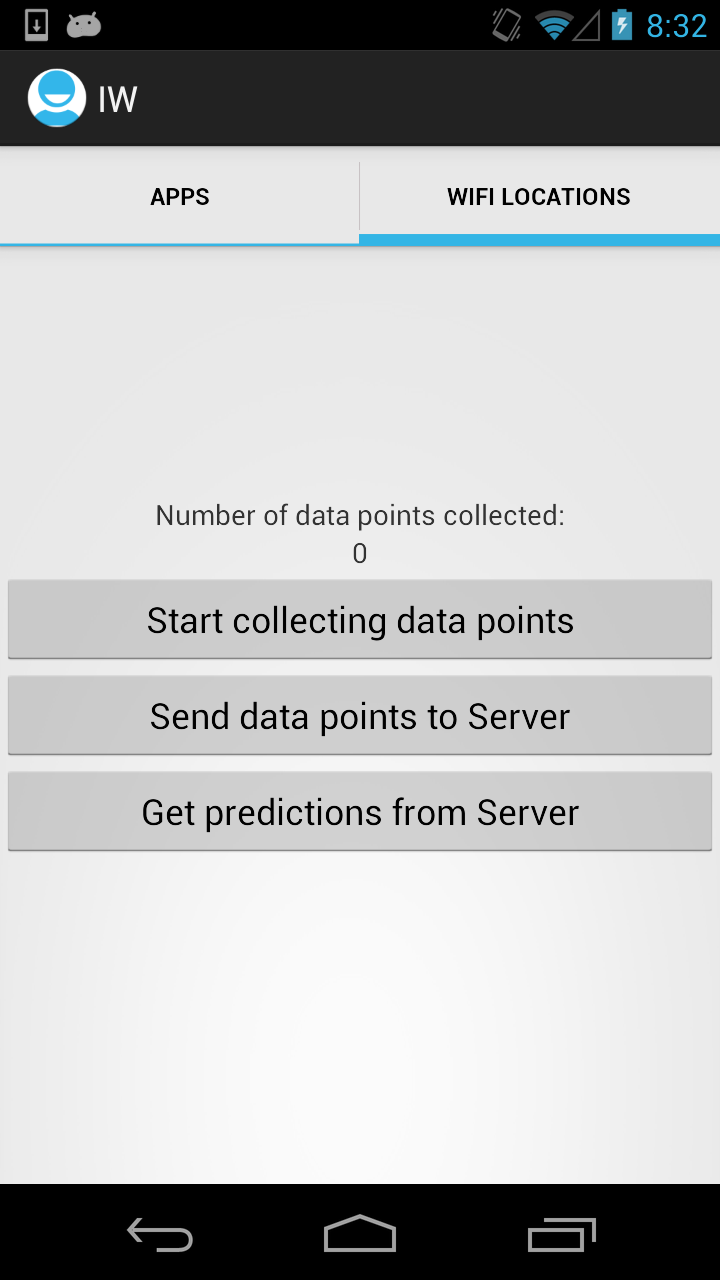
\includegraphics[scale=0.2]{img/app-screenshot-wifi.png}
\caption{App for collecting wifi and 3G data\label{fig-app-screenshot-wifi}}
\end{figure}
\medskip

\subsection{Server} 
\label{time-to-wifi-server}

At this point, the phone local store has stored values for the wifi and 3G network 
characteristics at different locations. Now, there is a question of where do we implement the machine 
learning algorithms that will leverage the data and predict the time-to-wifi. 
One solution would be to implement the algorithms on the phone itself. However, 
the phone's computation capacity may not be sufficient for machine 
learning algorithms - at any rate, it will be slower on the phone than a computer. It therefore makes 
sense to do it offline on a centralized server. This has the happy side-effect 
that it allows us to collaboratively use all users' collected data and hence 
get a better, denser mapping of wifi and 3G. 

Therefore, periodically, the values from the phone's local store are uploaded to a server. This is a server that I 
wrote on Google AppEngine, which basically has a script to receive 
data-points from the phone and store them in the very convenient AppEngine 
database. The app on the phone, when it is in range of wifi, pulls out data-points that it 
had stored in its local store, and makes a get request to this script to send data points to the 
server database. 

\medskip
\begin{figure}[htp]
\centering
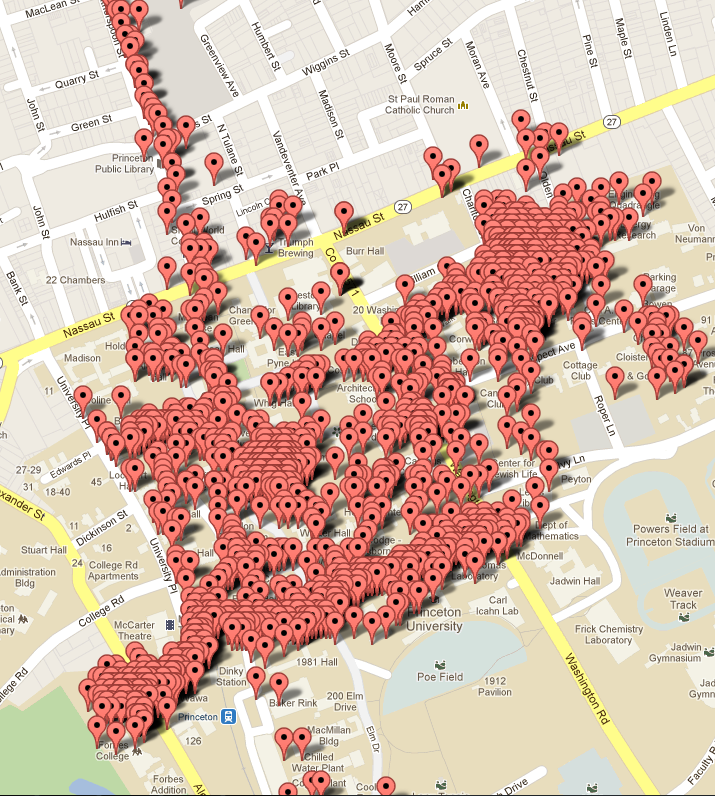
\includegraphics[scale=0.5]{img/map3033.png}
\caption{Collected data on the server - \texttt{http://cos598b.appspot.com/map}\label{fig-map-data}}
\end{figure}
\medskip

\subsection{Preprocessing of data}

Some steps were taken to ensure that the data was appropriate for analysis. We filtered
out all data points that were not accurate to at least 25m, since we expect wifi availability 
patterns to change significantly over that distance. Similarly, we filtered out data points that 
had speed of movement close to 0 m/s. The rationale for doing so is that if a user stood 
still at the same point for a while and then obtained wifi after some time, that time is not 
representative of how far that point would be from wifi if the user was walking. Lastly, we 
experimented with different locations and obtained a cut-off point for the wifi signal 
strength at which the internet connection is “good enough”. This solves the 
quality of service issue, and ensures that the wifi is of usable quality. Based on this cut-off point, 
and the wifi signal strengths for each data point, we recorded how long it took for each 
data point to obtain a strong enough wifi signal. We marked the time-to-wifi for points 
that did not obtain wifi within the 10 minutes as 10 minutes, for ease of analysis.

\subsection{Learning algorithms} 
\label{time-to-wifi-learning-algorithms}

The AppEngine server at this point has the preprocessed data-points of wifi and 3G 
characteristics at different locations. Note that these are stored 
for all users, and we collaboratively use all users' data-points in the 
learning algorithms described in this section. 

Intuitively, we want to look at the user's current movement patterns, 
correlate it with movement patterns in the past, and find the expected 
time-to-wifi. This is a prediction problem in continuous variables, and is a 
well-studied problem in machine learning and artificial intelligence. 
For this, we want to form a \textbf{prediction model}. This models 
the time-to-wifi as a \textbf{response} to (i.e. dependent on) some  
\textbf{covariates}. In our case, we model time-to-wifi as a response to 
covariates like location, bearing, speed etc. 

More concretely, we are collecting data points, which correspond to a certain 
location, bearing, speed, and timestamp. We also measure the time-to-wifi 
corresponding to each data point by looking at wifi signals for 10 minutes after 
the initial data collection. Our goal is to form a prediction model which, 
given a new data point (location, bearing etc), can predict the time-to-wifi corresponding to it. 
To form this prediction model, we used various machine learning techniques, as 
discussed in the following section. 

\subsection{Regression}
\label{time-to-wifi-regression}

Since we are dealing with continuous variables, regression immediately springs 
to mind to form the prediction model. 

\textbf{Linear regression}: Linear regression learns a linear model relating the 
response in terms of the covariates. It then uses this linear model to predict 
the response, given a new set of covariates. However, in our problem, 
it is expected that the wifi availability pattern at one location
could be completely different from another location. Similarly, the time-to-wifi could be 
vastly different even in the same location for two different bearings. Therefore, 
it is not possible to have a simple linear relation between the response (time-to-wifi) and 
the various covariates like location and bearing. For linearity, we divided location and bearing,
which were global variables, into sets of local variables instead.
We did this by dividing the map into a grid of blocks based on the GPS coordinates, 
and further subdividing each block into \textbf{sectors} based on bearing. For example, one sector 
could include all the data points that have their GPS coordinates in the square bounded by 
$(40.345, -74.660) - (40.350, -74.655)$ and bearing in the range $45^\circ$ - $90^\circ$. This
sector is shown in Figure \ref{fig-map-sector}.

\medskip
\begin{figure}[htp]
\centering
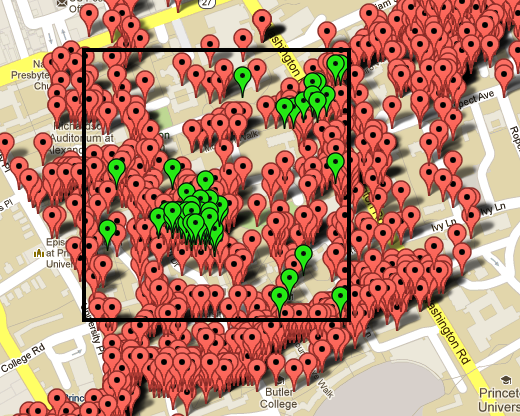
\includegraphics[scale=0.5]{img/map3033-sector.png}
\caption{Green points are one sector. They are the points in the bearing range $[0^\circ, 45^\circ]$ in the GPS coordinate square shown  (bounded by $(40.345, -74.660) - (40.350, -74.655))$. \label{fig-map-sector}}
\end{figure}
\medskip

We then performed cross-validated error analysis to see what granularity of 
dividing latitude/longitude and bearing into sectors yields best results. Cross-validation 
basically forms the prediction model based on \emph{part} of the dataset, and then 
uses this prediction model to predict time-to-wifi for the remaining part of the dataset. We can 
compare the predictions with the known values to find the error in prediction. 
By repeating this cross-validation for different sector sizes, we found that 
latitude/longitude divisions of $0.005^\circ$ and bearing divisions of $45^\circ$ work best.
 
Then, we modeled each data point as follows: each data point has some ``global" 
covariates like speed, timestamp associated with it. As described above, the ``global" variables
latitude, longitude and bearing were split up into sectors. Therefore, each data point also has 
three covariates per sector of the map. If the data point falls in a sector, 
then the values for its 3 covariates for that sector would be the latitude, 
longitude and bearing difference of the data point from the minimum bounds of 
that sector. If the data point does not belong to a sector, its 3 covariates 
corresponding to that sector have value 0. 

Then, using all the data-points from the past, we can come up with a linear model 
to predict time-to-wifi in terms of the many covariates. 

\bigskip
\textbf{Regularized regression}:	The same methodology as above was followed, except 
the model parameters/covariates were weighted via ridge regression. This allows 
us to penalize certain regression coefficients in a manner that reduces the variance in the 
prediction.

\medskip
\begin{figure}[htp]
\centering
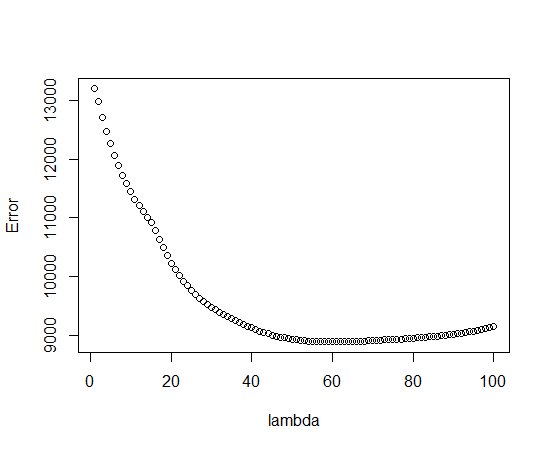
\includegraphics[scale=0.5]{img/ridge_lambda.png}
\caption{Cross-validated error vs. $\lambda$ for ridge regression\label{fig-ridge-lambda}}
\end{figure}
\medskip

To figure out the value of the ridge parameter $\lambda$, we found the cross-validated error
for various values of $\lambda$ (similar to method in linear regression). 
Figure \ref{fig-ridge-lambda} shows the plot of 
cross-validated error vs $\lambda$ as obtained from R’s \texttt{glmnet} package. Following the result of 
the graph, we used $\lambda = 60$ in our final analysis, since it shows minimum 
error. 

\subsection{$k$-means clustering}
\label{time-to-wifi-kmeans}

We use $k$-means clustering to form our prediction model. The general overview of the method is this:
we use $k$-means to split the training dataset into clusters, based on only the covariates 
(not the response). Then, for predicting time-to-wifi, we use the same covariates to assign 
the new datapoint to a cluster, and set its time-to-wifi to be the mean 
time-to-wifi of all training data-points in the cluster.

In our case, we expect that two data points originating close 
to each other and showing movement in the same direction would obtain wifi after 
approximately the same time. Hence, the covariates we used for $k$-means 
clustering were latitude, longitude and bearing (note that speed was not 
considered in this method). We also scaled down bearing by a factor of 18000 in 
order to make the variation in bearing approximately equal to the variation in latitude 
and longitude, since otherwise the clusters would form based simply on bearing (Note that 
across Princeton campus, latitude and longitude only changes by 0.02, compared 
to bearing which varies from $0^\circ$ to $360^\circ$). 

The time-to-wifi for each cluster was set to be the mean time-to-wifi of the data-points in 
that cluster. For predicting the time-to-wifi for a new data point, we find the cluster that it is
closest to, in terms of latitude, longitude and bearing, and set its 
time-to-wifi to be the mean value for that cluster. Similar to the cross-validation
in the previous sections, Figure \ref{fig-num-clusters} shows the plot of 
cross-validated error as a function of the number of clusters. 
%Surprisingly, the error continues to decrease even up until we have as many 
%clusters as data-points. Usually, one expects that the effect of overfitting would 
%become significant as the number of clusters is increased. However this plot suggests 
%that we did not have enough data points to observe overfitting. Clustering was eventually 
%chosen as the algorithm we implemented for the K-9 email client, because it showed 
%favorable results (Fig 4) and is practically efficient given the limited storage and 
%computational capabilities of a phone.

\medskip
\begin{figure}[htp]
\centering
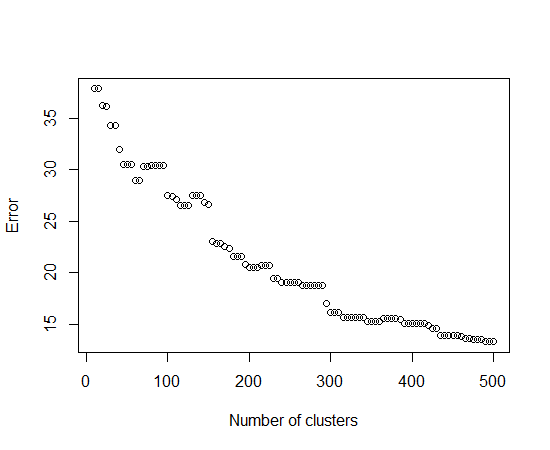
\includegraphics[scale=0.5]{img/num_clusters.png}
\caption{Mean cross-validated absolute error vs. number of clusters\label{fig-num-clusters}}
\end{figure}
\medskip

\subsection{Random forests}
\label{time-to-wifi-random-forests}

Once we realized that one of the major problems that we faced 
in terms of machine learning was sparseness of data (as described in Section \ref{time-to-wifi-analysis}), 
we looked for alternatives. One algorithm that we considered was random forests. 

Random forests builds up a forest of \emph{decision trees}. 
Decision trees are predictive models in themselves. They are a way of mapping the observations 
we see - location, speed, bearing - to the value that we want to learn - the 
time-to-wifi. Decision trees are best understood as following the path of making 
a decision based on the covariates. A part of such a decision tree is shown in the 
figure FIGURE

\textbf{TODO: figure about decision tree}

Therefore, a single decision tree can, given some value of the covariates, 
predict what the value of the time-to-wifi will be. However, the prediction 
depends entirely on the structure of the decision tree. Depending on the order 
in which we consider covariates going down the tree, or on whether we ignore 
certain covariates and emphasize others, we will get a different tree, and hence 
different predictions. This is where random forests comes in. It builds up a bunch 
of different decision trees using different splits of the covariates. 
Then, given a new data-point, it uses all these decision trees to make various 
predictions of time-to-wifi, and returns the average value found. 

We used random forests since it is quite effective with sparse data sets and it balances the error in datasets 
where the data are quite unbalanced, as is true in ours (again, further described in Section \ref{time-to-wifi-analysis}). 
This algorithm was quite easy to implement and analyze. We didn’t need to restrict the 
covariates as we did in linear regression because random forests itself can find the best split 
of covariates to use to base its decisions on. It also gives a measure of how important each 
covariate is, which is useful in analysis (notably, it showed that the speed measurement 
was not very important).

\subsection{Boosting}
\label{time-to-wifi-boosting}

Boosting is a predictive method that uses several weak predictors in conjunction 
to form a relatively strong predictor. Consider the situation where we have a 
few predictors of time-to-wifi that don't perform well, i.e. they have quite a 
lot of errors. Boosting can use these together and improve the overall 
performance. It is a fascinating algorithm, since it is guaranteed to predict the 
real value in the limit, as we increase the number of predictors. 

Boosting is something we tried more out of curiosity than anything. Since we 
had tried a few regression algorithms which had had a large error, we wondered if 
using boosting would help bring down the error by using multiple weak regression algorithms 
in conjunction. However, we found that boosting did not result in much 
better predictions, and in fact, in some cases it actually did poorer. 

\subsection{Testing and Analysis}
\label{time-to-wifi-analysis}

To test the value of using each of these algorithms, we used 5-fold cross 
validation. For this, first we split the training dataset into 5 parts. We  
train the prediction model on 80\% of the data. Using this model, we predict the time-to-wifi for 
the remaining 20\% of the data. Since the actual time-to-wifi for this 20\% is 
known, we can obtain the mean absolute error in prediction of time to wifi. The blue bars in Figure \ref{fig-error-outliers} 
show the results for each of the 5 algorithms. While random forest regression seems to 
perform significantly better overall than the rest, the errors are fairly high (35-70 seconds). We hypothesized 
that these errors could be due to the outliers in our data. These outliers could occur for 
two reasons:
\begin{enumerate}
  \item \emph{pathological movement patterns}: Firstly, users’ walking patterns can be non-uniform. For example,  
most people heading towards the CS building from the Shapiro Walk will obtain wifi in 
less than a minute. However, say a user who is taking this path suddenly 
remembers they have to go somewhere else, and end up turning away. The 
application will end up recording that the time-to-wifi along this path is much 
longer than it actually is. Consider what would happen if we were making our
prediction model using k-means. These “peculiar” data points, if clustered along with the more 
regular ones, can have predictions vastly different from the observed responses and 
hence skew our measure of average error. 

This source of error is more or less an unavoidable property of 
the problem we are trying to solve. The best we can do is to go ahead determine how long
to delay the app under the given prediction model.. If, during this delaying period, the application does 
not get wifi connectivity (perhaps due to misprediction), we can send the 
apps' network traffic over 3G instead.

  \item \emph{sparse data}: Secondly, as can be verified from Figure \ref{fig-map-data}, certain 
  areas have points that are more spatially separated. This sparseness of data means that we may 
not have enough information about the various possible movement patterns that a 
user could be walking along. This makes prediction hard, and hence can lead to high errors
under cross-validation. 

\begin{figure}[htp]
  \centering
  \subfloat{\label{fig-regression}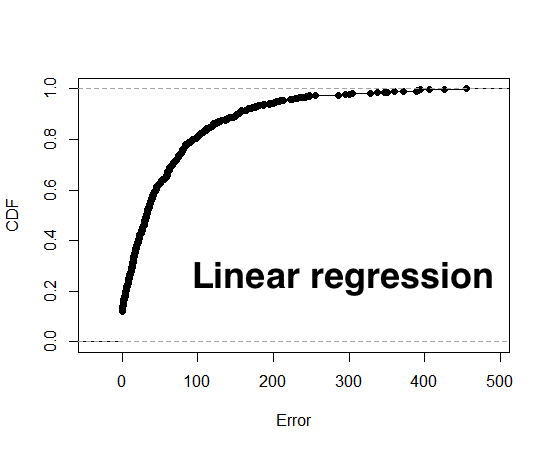
\includegraphics[width=60mm]{img/regression.png}}
  \subfloat{\label{fig-ridge}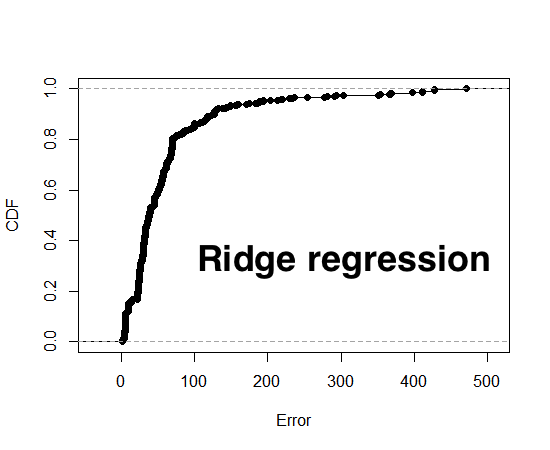
\includegraphics[width=60mm]{img/ridge.png}}
  \\
  \subfloat{\label{fig-boosting}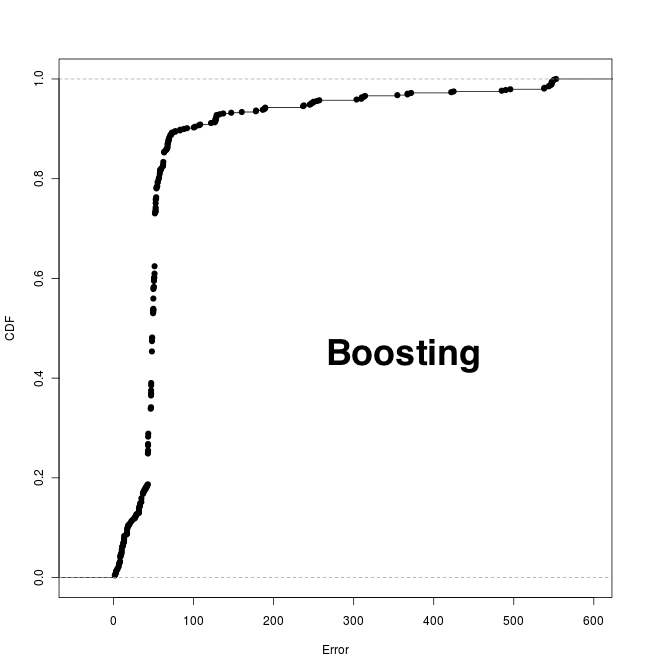
\includegraphics[width=60mm]{img/boosting.png}}
  \subfloat{\label{fig-clustering}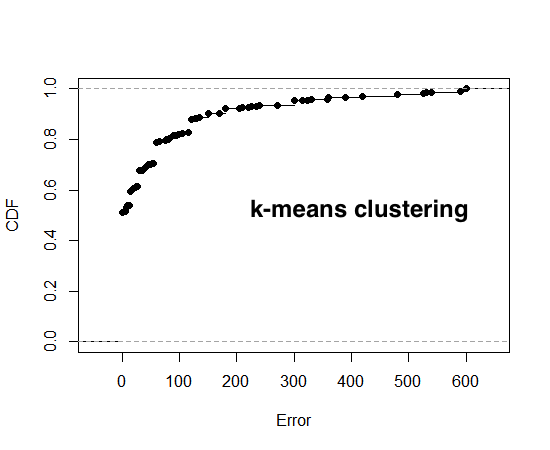
\includegraphics[width=60mm]{img/clustering.png}}  
  \\
  \subfloat{\label{fig-randomforest}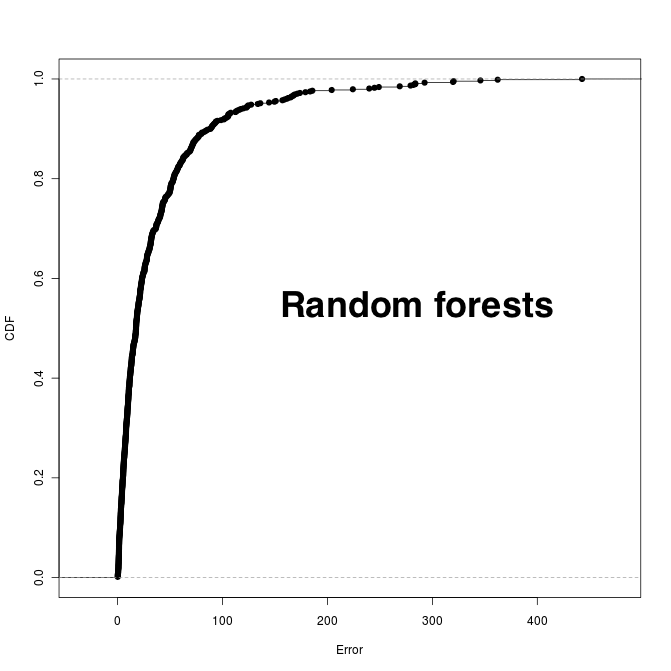
\includegraphics[width=60mm]{img/randomforest.png}}
  \caption{CDF of mean prediction errors for different algorithms \label{fig-cdf}}
\end{figure}

To find out if sparseness of data is an issue, I looked at the cumulative 
distribution (CDF) of the prediction error made by the different algorithms. This is 
reflected in Figure \ref{fig-cdf}. These CDFs show that the errors are more 
heavily weighted towards small errors, i.e. a large proportion of prediction 
errors are small. This is best seen in the CDF for random forests, where we can 
see that $\approx 80\%$ of the errors are on the order of 15 seconds. 

In order to further verify that average error was being skewed by a few large errors, 
we re-ran the algorithms, focusing only on the part of the campus 
where we managed to obtain a high density of data points (area around Friend Center, 
CS Building, ORFE, E-Quad, Shapiro Walk). Figure \ref{fig-error-outliers} shows the new results. Just as we expected, 
the average error decreases significantly to almost half of before, with all algorithms 
performing similarly well. This result indicates that we do not have enough data that is
distributed well over the entire campus. However, we believe 
that time-to-wifi estimator has significant value when it makes errors of $\leq 1$ 
minute,  which happens most of the time. Further, the predictions only seem to 
get better with increased density, and hence it is likely that we will get 
better results as more people use the system. 
\end{enumerate}

\medskip
\begin{figure}[htp]
\centering
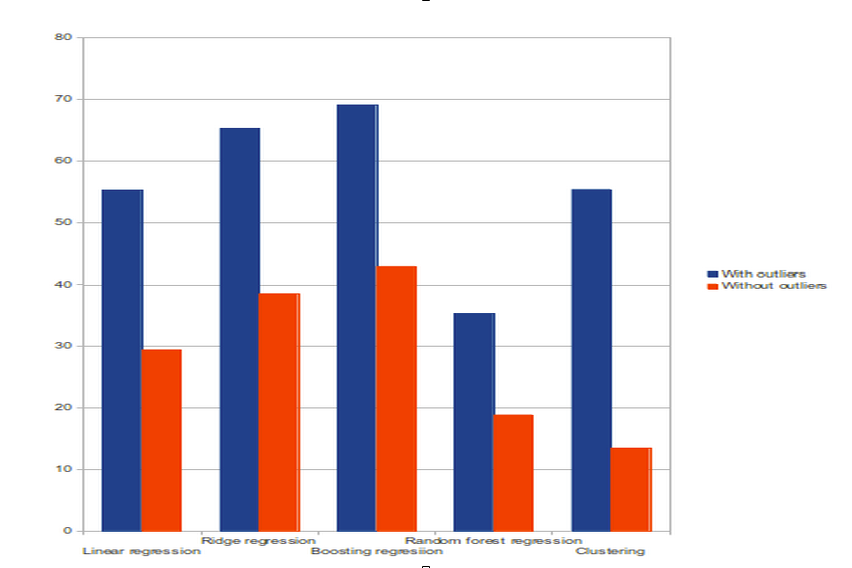
\includegraphics[scale=0.5]{img/error-outliers.png}
\caption{Mean cross validated absolute error for each algorithm (with and without outliers)\label{fig-error-outliers}}
\end{figure}
\medskip

\subsection{Prediction on the phone}
\labe{time-to-wifi-predict}

Now, we have used the data-points on the server to come up with a predictive 
model. We need to get the predictive model to the phone, and set up a way of 
using the model to predict time-to-wifi. For this, we firstly need a convenient
way to represent a predictive model. This is quite easy to do, and in fact, most 
machine learning packages provide a way to output the predictive model in 
an easy-to-use format. For example, for $k$-means clustering, we only need 
to keep track of the centers of the clusters, and their corresponding time-to-wifi values.

We can then co-opt the same data collection app described above (Section \ref{time-to-wifi-data-collection}) 
to receive the predictive model from the server, using a simple HTTP request to fetch a \texttt{.txt} file. 
For space-efficiency, we only send that part of the predictive model which corresponds 
to the user's current location and nearby areas (since the predictive model for the entire
world can be quite large). This app exposes this predictive model through a method 
which can be called to predict the time-to-wifi, given the user's current location, bearing etc. 

In summary, the app collects the data for learning the predictive model, and 
sends this data to a server. Machine learning algorithms run on the server to 
form a predictive model, which is sent back to the same app. This app then acts 
as the time-to-wifi predictor through an interface with the rest of the 
applications.

\subsection{Future Improvements}

In the future, the following improvements could be made to the time-to-wifi 
predictor:
\begin{itemize}
  \item In making the time-to-wifi predictions, we use all users' 
  data-points of wifi and 3G locations, and we consider 
  each user's data to be equal. Maybe in the future we could weight the 
  current user's data a little more in making predictions, since it more likely 
  to reflect the user's movement patterns.

  \item The current solution requires machine learning to be done offline on a 
  server - this was because it would be easier to program and also faster. 
  However, a more realistic solution would probably use some greedy online heuristics on 
  the phone to learn time-to-wifi on the fly as network requests are being 
  made (instead of needing a pre-computed prediction model).
  
  \item For measuring time-to-wifi, we are currently using wifi signal strength 
  as an indication of how usable the wifi signal at a given point is. However, 
  various papers have shown that signal strength is a poor predictor of wifi 
  quality. We currently use it in the system out of ease of programming. 
  Ideally, however, we should test wifi quality by doing some sort of bandwidth 
  test. This could involve sending small packets of data to ping a known server 
  and waiting for a response. This empirical method would help us more 
  accurately gauge the quality of wifi.
\end{itemize}

%%%%%%%%%%%%%%%%%%%%%%%%%%%%%%%%%%%%%%%%%
%%%%%%%%%%%%%%%% SECTION %%%%%%%%%%%%%%%%%%
%%%%%%%%%%%%%%%%%%%%%%%%%%%%%%%%%%%%%%%%%

\section{Application delay tolerance estimator}
\begin{itemize}
\item Data collection - app screenshot
\item Current solution
\item Results
\item Future improvements: Not just poll every so often, but update traffic stats 
every network request (disadv: requires kernel access?)
\end{itemize}

The other input into the policy is the application delay tolerance estimator. 
Just to recap, this estimator will learn from the apps' past network usage statistics - 
how much data does each app send, and what is the usual pattern of this data 
generated. We expect, for example, that a video streaming app would be show
constant, high-bandwidth pattern, as contrasted to a web browser where we would 
expect more bursty, low size traffic as the user clicks around on links.

Then, when we see a certain app making network requests we can look at its past network 
patterns to gauge its delay tolerance. This will be an input into the policy.
 
\subsection{Data collection}

\begin{figure}[htp]
\centering
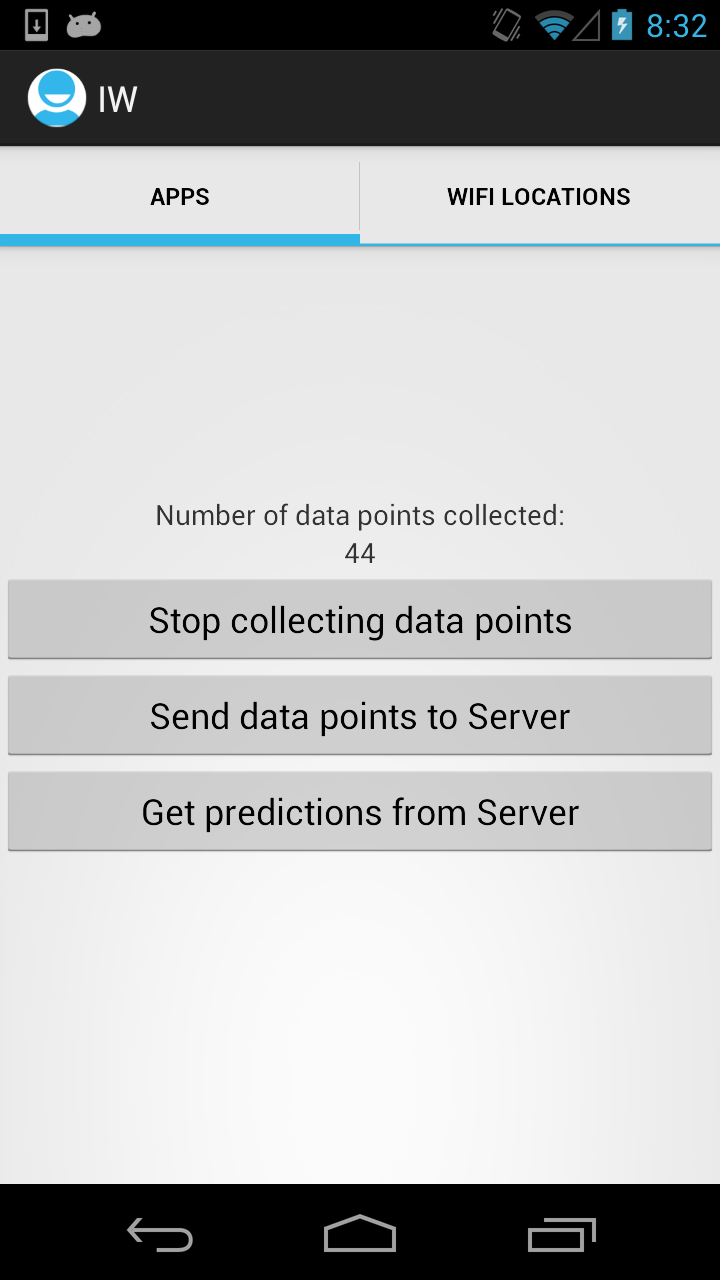
\includegraphics[scale=0.2]{img/app-screenshot-apps.png}
\caption{App for collecting network usage statistics of other apps \label{fig-app-screenshot-apps}}
\end{figure}
\medskip

For the delay tolerance estimator, we first need to collect data about the 
network usage of all apps. For this, I built another app that runs on the phone 
in the background and records apps making network requests, storing the 
network usage statistics of each app at different times. 

This app uses the \texttt{TrafficStats} class which exposes the following four different network 
data statistics for each app:
\begin{enumerate}
  \item number of bytes sent over TCP
  \item number of bytes sent over UDP
  \item number of bytes received over TCP
  \item number of bytes received over UDP
\end{enumerate}

The app periodically polls the \texttt{TrafficStats} class and records the above
values for all the apps at that time. NB: if an app's network stats have not 
changed at all since the previous recording, meaning that it has had no network 
activity in the intervening time, then we don't record its value again, to avoid 
redundancy. 

We can see that this quantizes the network traffic pattern graph. If we make the 
first record from \texttt{TrafficStats} at time $t_1$ and then the second at 
$t_2$, then we are attributing all the network traffic in the interval $(t_1, t_2]$ 
to time $t_2$. However, if our \texttt{TrafficStats} sampling is done frequently 
enough, then we will approach a quantization level where it will be imperceptible to the 
user. We chose a sampling rate of 100 ms, which is fine because we will be 
calculating delay tolerance in the order of seconds and so this is an order of 
magnitude better resolution.  

\subsection{Learning delay tolerance}

In trying to learn the delay tolerance of apps, the question arose as to whether to do the machine learning on the phone 
rather than the server. Initially, we attempted to follow a method similar to that
used to find the time-to-wifi - doing offline learning on the server to form a compact 
prediction model on the phone. While this method seemed more rigorous, it was
quite hard to implement algorithms to learn delay tolerance. However, a key insight
showed us that the learning of delay tolerance could be a matter of simple statistical 
analysis, and hence could be done on the phone. We can sample all the network
statistics collected by the app described above, and analyze these in an \emph{online} 
manner. This means that the amount of data stored is always a constant amount, 
and we need not make expensive requests to send data-points to the server, and 
receive prediction models from the server. 

So how do we actually do all this on the phone? 
We now know the network statistics of all apps running on the phone. Using this 
information, we want to determine the apps' delay tolerance.  When a user is 
directly interacting with an app, any network traffic generated is not delay 
tolerant. This is obvious - we cannot delay traffic that the user is explicitly
waiting for without adversely affecting their interaction and experience with the app. 
Therefore, we discard statistics about these situations. From the 
remaining stats, we can find out the \texttt{GET} requests made by the app in the 
\emph{background}. For applications like email clients and messengers, these 
background requests tend to be requests for background syncing. As we have 
already discussed at length, such network requests are usually tolerant to delay 
as long as the user isn't directly interacting with the app making the request. 

\medskip
\begin{figure}[htp]
\centering
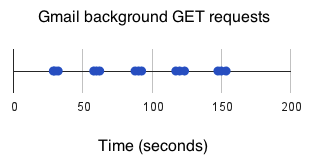
\includegraphics[scale=1.0]{img/dt-get-req-gmail.png}
\caption{Background GET requests sent by Gmail app \label{fig-dt-get-req-gmail}}
\end{figure}
\medskip

So, now that we know that what sort of traffic we can actually delay, we want to be able to figure
out how long we can delay the network traffic for, i.e. what is the delay tolerance of the traffic. 
Figure \ref{fig-dt-get-req-gmail} shows background \texttt{GET} requests for the 
Gmail client, whose background traffic I logged. It shows that the app 
sends out syncing requests every so often as a \emph{cluster} of 3-4 separate \texttt{GET} requests. 
Note that these multiple near-simultaneous requests are not retransmissions. Rather, they all serve
different purposes: for e.g. on the email app, these are multiple concurrent requests 
to refresh the various different email folders. Also note that the fact that we 
are logging network statistics only every 100 milliseconds or so does not affect 
these \texttt{GET} requests. This is because the \texttt{GET} requests are separated by seconds 
rather than milliseconds.

The time between these successive requests is an indication of how much the app 
is willing to wait before pinging for updates. This is in line with our 
definition of delay tolerance: if the app is willing to wait one minute before 
sending a background sync request, then that must mean that it's background 
network requests are tolerant to delays on the order of one minute. 
Note that this pattern seems to be true in the background usage 
statistics of other apps as well - I looked at K9, an open-source email app, and 
Facebook as well. <DRAW GRAPH FOR THESE APPS>

In the context of the \texttt{GET} request graph shown above, we can come up
with a method for actually gauging delay tolerance. To learn delay tolerance of an app, we should 
look at the time periods between the clusters of requests. This means that we should
consider the clusters of concurrent requests as one single request. Naively, 
this is quite simple to do. We can simply store the timestamp of the last \texttt{GET} 
request sent by the app. Then, when a new background \texttt{GET} request is sent, 
we can subtract the stored timestamp value from the current time to get an
estimation of delay tolerance. 

However, there are improvements which can be made to this method. First of all, 
we can see that we are recalculating delay tolerance every time, and we don't 
end up making full use of the history of the app's network usage. If we simply 
follow the method above of subtracting the past timestamp from the current, we 
have a model that is only looking at the past two time steps and discarding
the rest of the information about the past. Rather than doing 
so, we can calculate delay tolerance as a time-weighted average of the time 
differences we are recording. Mathematically, we can define this recursively as 
follows:
\begin{equation} \label{eq-dt-weighted-avg}
  D_i = \lambda \Delta t_i + (1 - \lambda) D_{i-1}
\end{equation}
where $\lambda$ is the weight for taking the average (the higher the value of 
$\lambda$, the more we weigh recent observations as compared to past 
observations). To unpack this equation a bit more, we are calculating the $i^\textrm{th}$ 
estimate of delay tolerance using the weighted average of 1) the $(i - 1)^\textrm{th}$ 
estimate of delay tolerance, and 2) the time between the two most recent \texttt{GET} requests.

So far, we have assumed that \texttt{GET} requests are infrequent, periodic, single pings. 
However, in reality as we saw above, apps tend to send out a cluster of separate \texttt{GET} 
requests close together. We need to be able to account for this. Intuitively, this will 
require us to ignore or discount \texttt{GET} requests if another \texttt{GET} request was 
made by the same app very recently. If we choose to \emph{discount} them, then we can simply 
have a threshold on the amount one \texttt{GET} request can change the delay tolerance estimate. 
For example, we can say that a single request can only change the delay tolerance 
by at most $\pm 10\%$, and clamp any bigger changes to this maximum value. On 
the other hand, we can also \emph{ignore} \texttt{GET} requests that come too 
close together. Therefore, if we see many requests coming together, we can 
ignore all but one of them, i.e. we can cluster them together. To do this, we 
can see when two \texttt{GET} requests are closer together than a minimum 
fraction of the current delay tolerance estimate, i.e. if
\begin{equation} \label{eq-dt-clustering}
  \frac{\Delta t_i}{D_{i-1}} < \epsilon
\end{equation}
we can ignore $\Delta t_i$ in the delay tolerance calculation.

In summary therefore, we have uncovered three (related) methods to gauge delay tolerance:
\begin{enumerate}
  \item \emph{Basic method:} Simply take the weighted average of current delay 
  tolerance estimate and the time between last two \texttt{GET} requests (see Equation \ref{eq-dt-weighted-avg})
  \item \emph{Clamping} the change in delay tolerance estimates to some maximum 
  factor, say 10\%. 
  \item \emph{Clustering} requests that are close together by ignoring all but one of them. 
\end{enumerate}

Note that these are online algorithms, i.e. they examine the stream of 
data as it comes in, but only store a constant amount in order to make their 
estimates.

\subsection{Results and Analysis}

\medskip
\begin{figure}[htp]
\centering
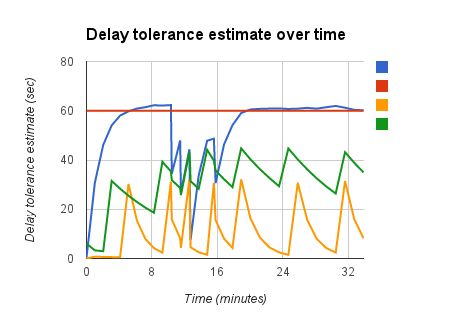
\includegraphics[scale=1.0]{img/dt-vs-time.png}
\caption{Estimation of delay tolerance \label{fig-dt-vs-time}}
\end{figure}
\medskip

We now move to discussing the relative merits and demerits of the three methods 
of learning delay tolerance. Above is a graph which shows the delay tolerance 
estimates made over time by the three methods, compared with the real delay tolerance
of 60 seconds. These measurements were made for the open-source K9 email client.
\begin{enumerate}
  \item The basic method (orange line in Figure \ref{fig-dt-vs-time}) is a naive method. It assumes that background sync 
  occurs through a single network request. However, in reality, quite a few packets are sent 
  together. Since these have very short intervals between them, it brings down 
  the delay tolerance estimate greatly. This is reflected in the valleys in the above
  graph, where the delay tolerance estimate goes down quickly due to many 
  \texttt{GET} requests. The steep climb thereafter is due to the fact that the 
  app waits and doesn't send any \texttt{GET} requests after sending out sync requests 
  for the first time.
  
  However, it is interesting to note that, as a result of this method's naivete, 
  it ends up considering all \texttt{GET} requests, and so it is guaranteed to 
  always be bounded from above by the true frequency of background syncing (the red line). 
  Therefore, we are always underestimating delay tolerance and erring on the side 
  of caution. On the other hand, we are not able to delay packets as much since 
  the delay tolerance is lowered.  
  
  \item The method of clamping (green line in the graph) helps reduce the effects of multiple requests 
  coming in together. Since each of these requests can only change the delay 
  tolerance estimate by at most 10\%, we don't see as much of a drop as we saw 
  with the basic method. 
  
  However, even 4 requests coming in together would result in a drop down to 
  65\% of the original value, and as a result, we can see that this method also 
  underestimates the delay tolerance value, albeit not as much as the basic 
  method.
  
  \item Instead, if we just cluster the concurrent requests together, we get the 
  red line in the graph above. This method does much better at 
  predicting delay tolerance. Since it considers only the time between 
  subsequent syncing requests, it provides a good approximation of the real 
  frequency of background syncs. As we can see in the graph, the estimate of 
  delay tolerance stabilizes around the value of 60 seconds.
  
  Note that this method also has its pitfalls. It depends on a good selection of $\epsilon$ 
  as defined in Equation \ref{eq-dt-clustering}. If the value of $\epsilon$ is 
  too low, we will end up considering \texttt{GET} requests that we should have 
  ignored. In fact, if we look at Figure \ref{fig-dt-vs-time}, this is precisely 
  what we see from $x \approx 10$ to $x \approx 20$. Here, the \texttt{GET} 
  requests came close together, but not close enough to be clustered together according to 
  Equation \ref{eq-dt-clustering}. Therefore, we end up getting a low estimate of 
  delay tolerance before it settles back to the real value. 
  
\end{enumerate}

\subsection{Future work}

The following improvements could be made in the future to the delay tolerance 
estimator:

\begin{itemize}
  \item As we have described above, the data collection app quantizes time. It 
  only polls for changes in network stats every 100 milliseconds or so, and 
  therefore, ends up having a coarse-grained idea of when apps actually send and 
  receive data. Instead, if we could actually look at the network requests as 
  they happen, we would have a better estimate of delay tolerance. Our initial 
  reservation against doing this was over the fact that it would require working 
  in the kernel in the network stack. However, as described in Section 
  \ref{mechanism}, I had to fiddle with the network stack anyway for another purpose.
  Therefore, it should now be easy to implement the data collection app for the 
  delay tolerance estimator in the kernel and get more precise measurements. 
\end{itemize}


%%%%%%%%%%%%%%%%%%%%%%%%%%%%%%%%%%%%%%%%%
%%%%%%%%%%%%%%%% SECTION %%%%%%%%%%%%%%%%%%
%%%%%%%%%%%%%%%%%%%%%%%%%%%%%%%%%%%%%%%%%

\section{Mechanism}
\label{mechanism}

At this point, we have built the 2 machine learning components which provide the 
time-to-wifi and delay tolerance estimates. Using these, we can construct a 
policy which will inform us about how much to delay network traffic. However, 
before we delve into this, let us consider a mechanism for delaying 
traffic, i.e. some actual code that runs on the phone to delay network packets for 
some requisite amount of time. As explained in Section \ref{overview-approach}, 
we want to implement the mechanism in the network stack in the kernel, so as to 
avoid requiring application developers from changing their apps in any way. 

Therefore, the general approach is to insert ourselves in the network stack, so 
that we can examine all network requests that are being made. If we find that 
wifi is not available when trying to make a network request, we can ask the 
policy whether that request can be delayed, and if so, how long it can be 
delayed for. Since we are in the network stack at this point, we can  
delay the network request in the hopes of getting wifi soon, and if successful, 
we can send the request out over wifi. However, if the delaying timer expires 
without us getting in range of wifi, we will just send the request over 3G so as 
to not affect the user experience. 

\subsection{Serval}
\label{mechanism-serval}

Serval is a project of a networking group at Princeton University led by Michael 
Freedman. The project aims to modify the network stack to allow for 
service-centric networking, i.e. networking set up around network ``flows" 
between the user and the service they are using. These flows account for 
dynamism (e.g. due to user mobility) and multiplicity (e.g. due to multiple interfaces at the user end)
in the networks underlying these services. This was not previously possible in 
the traditional host-centric TCP/IP stack. They introduce a Service Access Layer 
(SAL) on top of this traditional network stack, which allows applications to 
interact over service names (instead of hostnames). 

As a part of their modifications to the network stack, they introduced 
mechanisms to allow for migration of network flows from one interface to 
another. We can see how this would be useful for service-centric networking - it 
allows a flow to continue uninterrupted even if the user is moving around and 
switching from wifi to 3G, or between various wifi access points. We can co-opt 
this mechanism in Serval to allow us to switch between wifi and 3G, for example 
if we delay a network request that was going to be sent over 3G and end up getting
wifi before the delay timer expired.

Ozlem Biglir Yetim, as part of her own research described in Section \ref{related-work}, 
introduced another mechanism into Serval which allowed for the delaying of 
network flows. This is again useful for our work, since we need to delay network 
requests according to the policy if wifi is not available.

\begin{figure}[htp]
  \centering  
  \subfloat{\label{fig-serval-delay}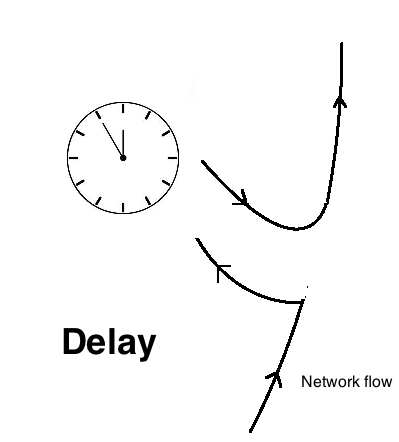
\includegraphics[width=70mm]{img/mech-delay.png}}
  \subfloat{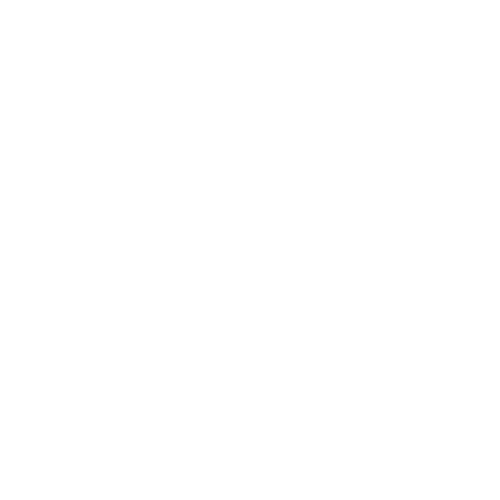
\includegraphics[width=40mm]{img/white.png}}
  \subfloat{\label{fig-serval-migrate}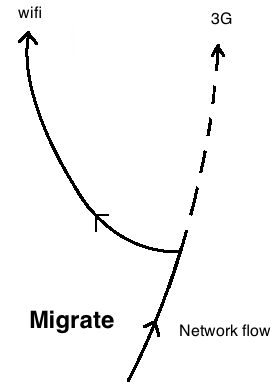
\includegraphics[width=50mm]{img/mech-migrate.png}}
  \\
  \caption{Serval can be used for delaying network flows and migrating them across interfaces. \label{fig-serval}}
\end{figure}


Because of these delaying and migration mechanisms, and also because working with
the SAL codebase would allow me to immediately enter the network stack, I
decided to use Serval to implement the mechanism. It was relatively 
straightforward to modify SAL to allow us to look at every network request. 
If wifi wasn't available, we could use the policy to figure out how long 
to delay the request, and delay it accordingly using functions already existing in the codebase.  

%%%%%%%%%%%%%%%%%%%%%%%%%%%%%%%%%%%%%%%%%
%%%%%%%%%%%%%%%% SECTION %%%%%%%%%%%%%%%%%%
%%%%%%%%%%%%%%%%%%%%%%%%%%%%%%%%%%%%%%%%%
 
\section{Overall policy}

\begin{itemize}
\item "The goal is to 
  compare the performance of different policies in different settings (for 
  example, settings where wifi and 3G are geographically well mapped out, as compared to 
  settings where they are not)."
\end{itemize}

Plan:
\begin{itemize}
  \item Just walk around with the phone with k-9 running, with 3G and wifi, and 
  see how many delays actually happen, and how many are successful.
  \item Log this in a way such that it is policy independent. For example, you 
  can record when the delay prediction was made, how much it was delayed, and 
  how much time it actually took to wifi (note that if we don't get wifi by the 
  time the delay tolerance runs out, we switch to 3G always) - this method of 
  recording data will allow us to analyze different policies using the same 
  dataset, e.g. a policy which delays if time-to-wifi < delay tolerance, or a 
  policy which delays for fixed 10 sec can both be tested using this dataset.
  \item Try to come up with different policies
  \item As you're finishing up, try to look for papers for each of the points - 
  e.g. wifi power level measurement using signal strength, papers on wifi vs 3G 
  battery consumption. Basically look for previous work on anything that I've 
  done, like using learning to predict movement patterns (specifically Markov 
  models).
\end{itemize}


%%%%%%%%%%%%%%%%%%%%%%%%%%%%%%%%%%%%%%%%%
%%%%%%%%%%%%%%%% SECTION %%%%%%%%%%%%%%%%%%
%%%%%%%%%%%%%%%%%%%%%%%%%%%%%%%%%%%%%%%%%

\section{Experiments}

%%%%%%%%%%%%%%%%%%%%%%%%%%%%%%%%%%%%%%%%%
%%%%%%%%%%%%%%%% SECTION %%%%%%%%%%%%%%%%%%
%%%%%%%%%%%%%%%%%%%%%%%%%%%%%%%%%%%%%%%%%

\section{Results}

%%%%%%%%%%%%%%%%%%%%%%%%%%%%%%%%%%%%%%%%%
%%%%%%%%%%%%%%%% SECTION %%%%%%%%%%%%%%%%%%
%%%%%%%%%%%%%%%%%%%%%%%%%%%%%%%%%%%%%%%%%

\section{Conclusions}

%%%%%%%%%%%%%%%%%%%%%%%%%%%%%%%%%%%%%%%%%
%%%%%%%%%%%%%%%% SECTION %%%%%%%%%%%%%%%%%%
%%%%%%%%%%%%%%%%%%%%%%%%%%%%%%%%%%%%%%%%%

\newpage
\begin{thebibliography}{9}
  \bibitem{att-coverage}
    AT&T 3G coverage in USA,
    $<$http://www.wireless.att.com/coverageviewer/#?type=data$>$.
  
  \bibitem{att-data-plans}
    AT&T data plans, 
    $<$http://www.att.com/shop/wireless/data-plans.html$>$.
    
  \bibitem{lee-2012}
    Lee, Kyunghan, Joohyun Lee, Yung Yi, Injong Rhee, and Song Chong, 
    ``Mobile Data Offloading: How Much Can wifi Deliver?"
    \emph{IEEE/ACM Transactions on Networking}, 
    Philadelphia, USA
    June 2012.
    
  \bibitem{raman-2007}
    Raman, Bhaskaran and Kameswari Chebrolu,
    ``Experiences in Using WiFi for Rural Internet in India."
    \emph{IEEE Communications Magazine},
    January 2007: 
    104-110.  
     
  \bibitem{verizon-coverage}
    Verizon 3G coverage in USA,
    $<$http://opensignal.com/network-coverage-maps/verizon-coverage-map.php$>$.
    
  \bibitem{verizon-data-plans}
    Verizon data plans,
    $<$http://www.verizonwireless.com/wcms/consumer/shop/share-everything.html$>$.
  
  \bibitem{yetim-2012}
    Yetim, Ozlem Bilgir, and Margarent Martonosi,
    ``Adaptive Usage of Cellular and wifi Bandwidth: An Optimal Scheduling Formulation."  
    \emph{CHANTS '12}, 
    Istanbul, Turkey, 
    August 22, 2012.
  
\end{thebibliography}


\end{document}
